\chapter{Tests}

\section{Schematics}

float barrier command to ensure that text stays close to the picture but no text from after the picture.

\subsection{part 1}

\begin{figure}[ht]
    \centering
    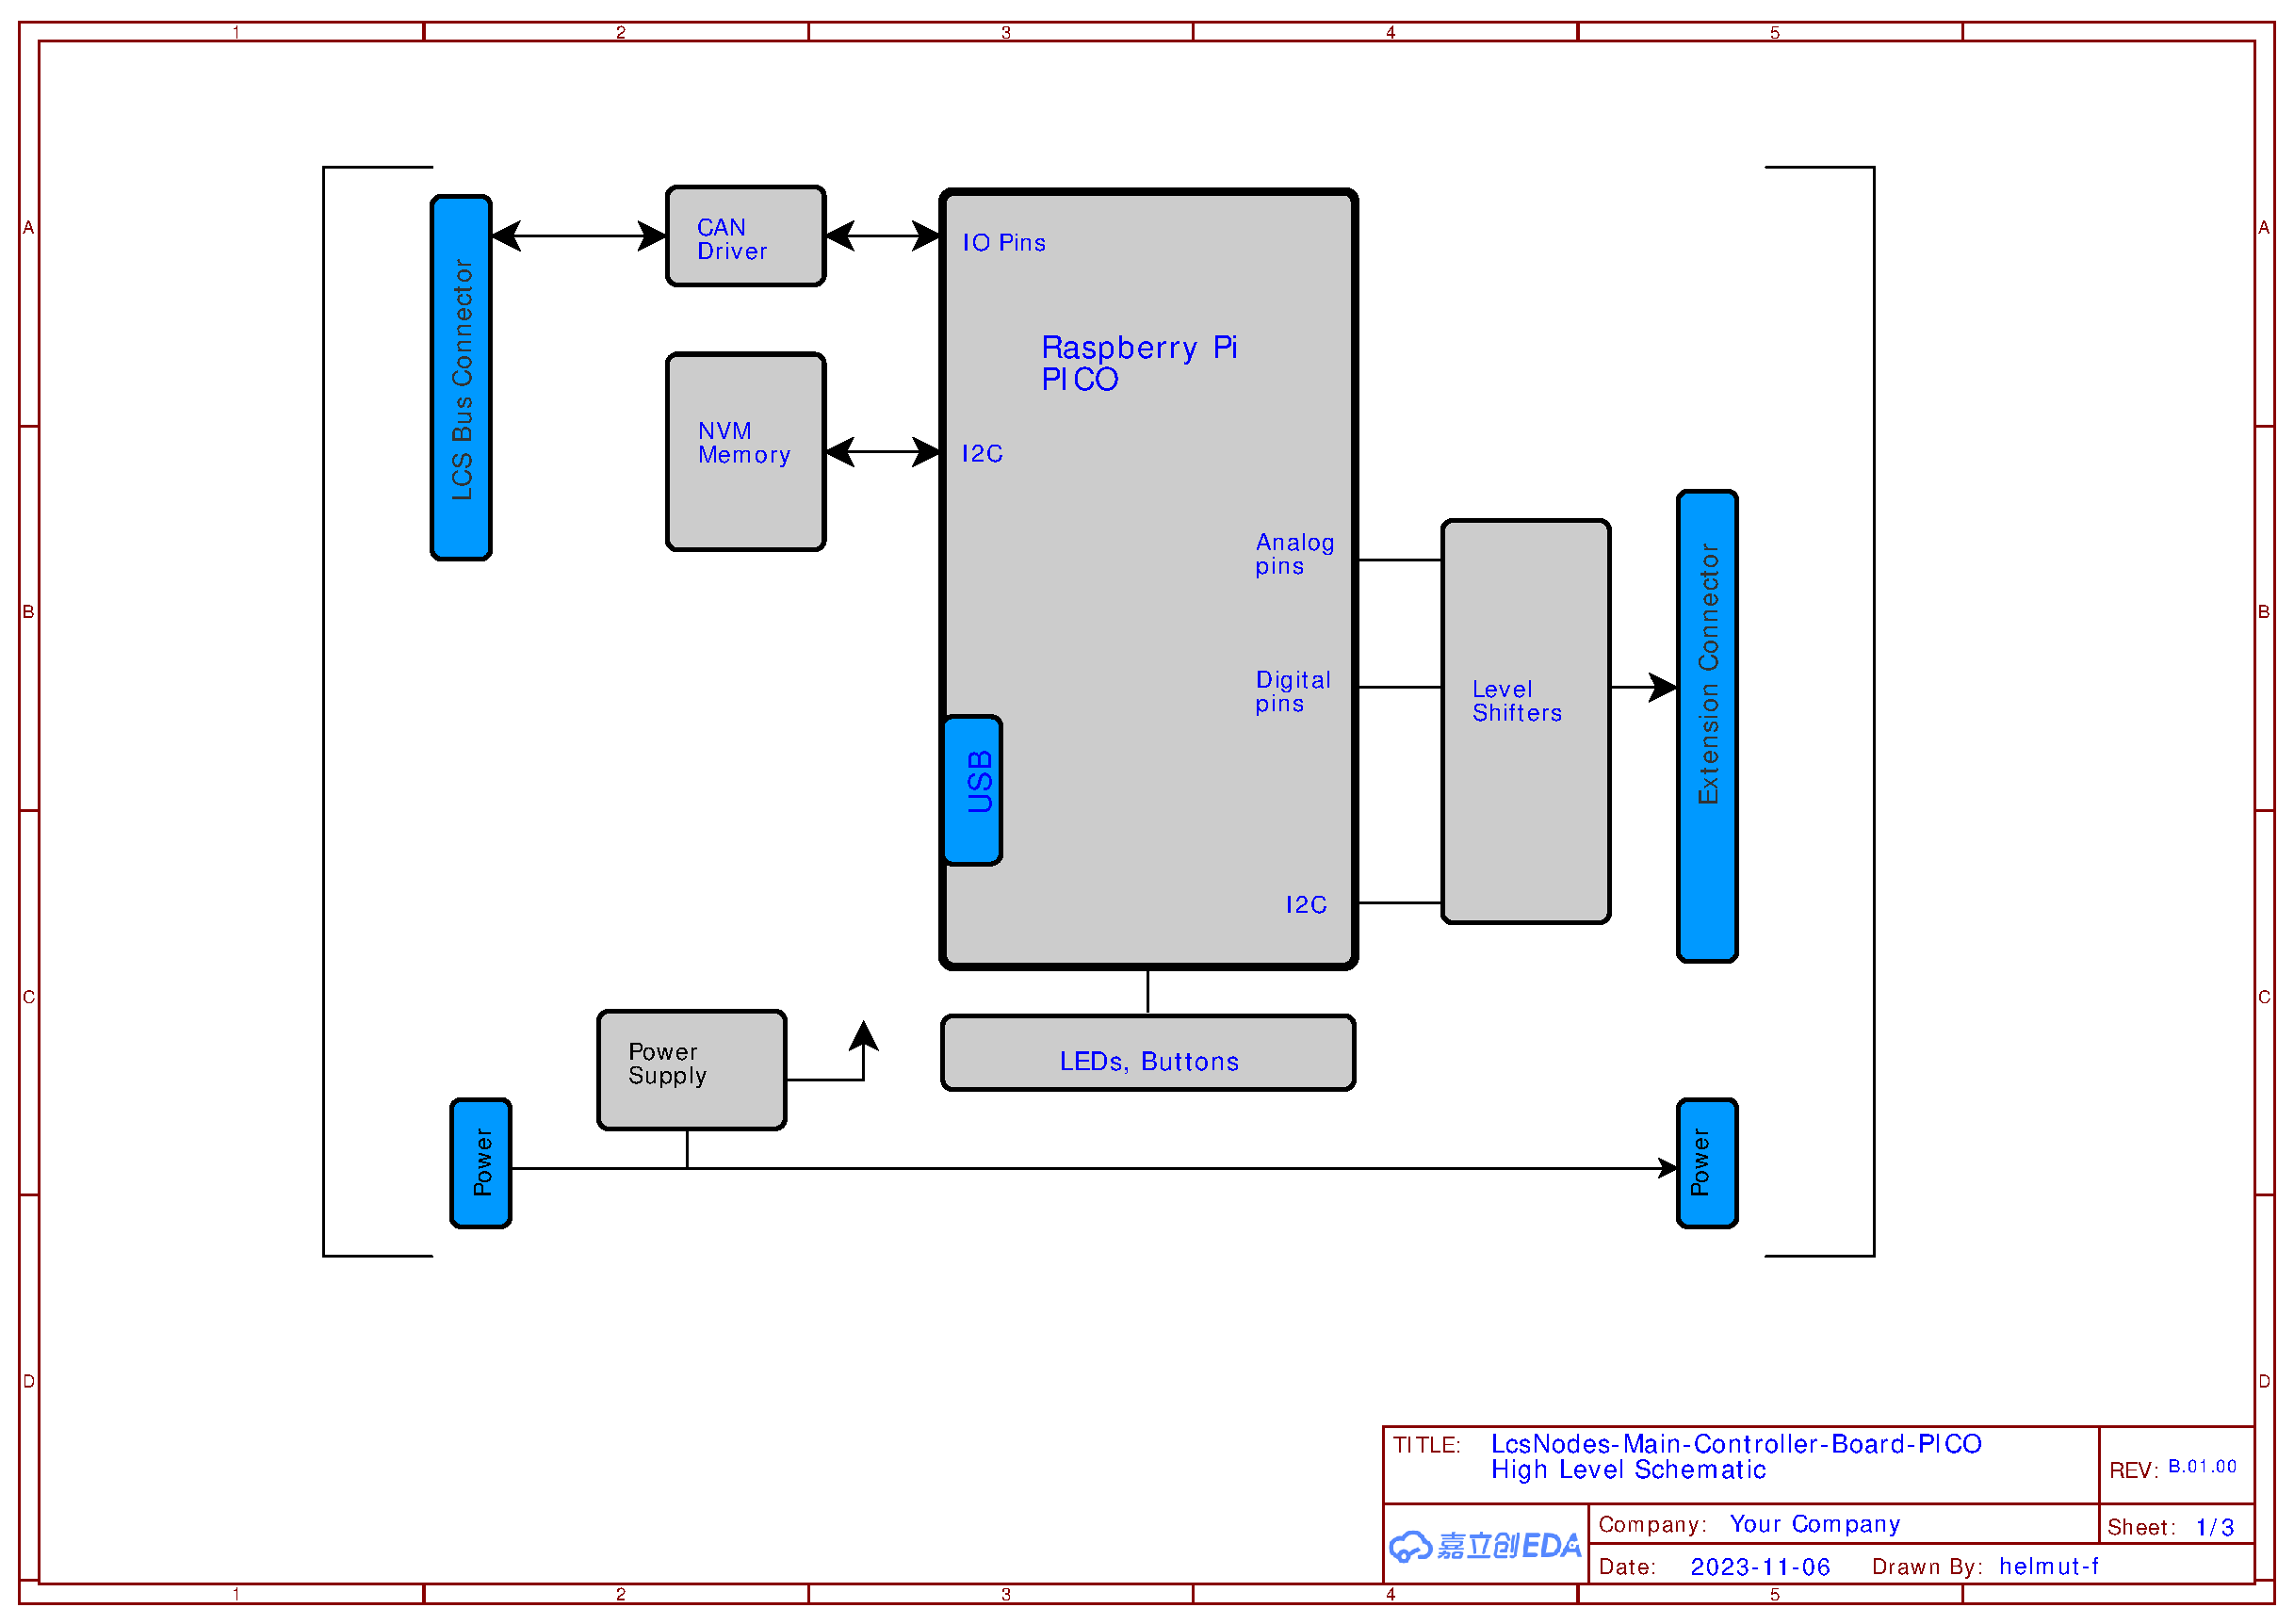
\includegraphics[page=1, width=\textwidth]{./schematics/Schematic_LcsNodes-Main-Controller-Board.pdf}
\end{figure}

\FloatBarrier

\subsection{part 2}
\begin{figure}[ht]
    \centering
    \includegraphics[page=2, width=\textwidth]{./schematics/Schematic_LcsNodes-Main-Controller-Board.pdf}
\end{figure}

\FloatBarrier

\subsection{part 3}
\begin{figure}[ht]
    \centering
    \includegraphics[page=3, width=\textwidth]{./schematics/Schematic_LcsNodes-Main-Controller-Board.pdf}
\end{figure}

\FloatBarrier


\section{Pictures}

\subsection{Variable word layout}

A little test for a word layout ... will be a bit fiddling work ... 

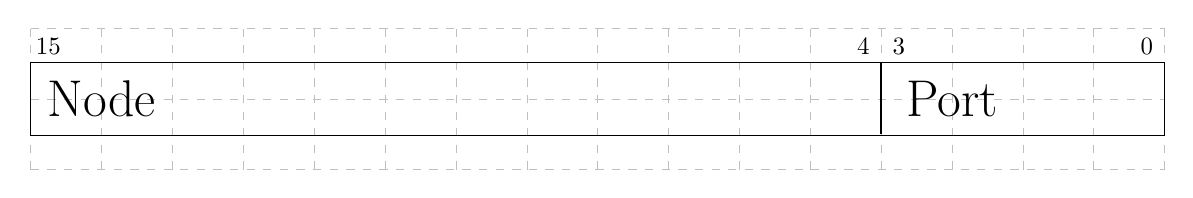
\begin{tikzpicture}[scale=0.9, transform shape]

    \draw[help lines, gray!50, dashed] (0,0) grid( 16,2);
    
    \node[  draw, 
            rectangle, 
            minimum width=16cm, 
            minimum height=0.8cm, 
            text height=0.8cm, 
            align=left] (A) at (8, 1) 
            { };

    \draw[thick] (12, 0.5) -- (12, 1.5);
    \node[above] at (0 + 0.25, 1.5) {15};
    \node[above] at (12 - 0.25, 1.5) {4};
    \node[above] at (12 + 0.25, 1.5) {3};
    \node[above] at (16 - 0.25, 1.5) {0};
    
    \node at (1, 1) {\huge Node}; 
    \node at (13, 1) {\huge Port}; 

\end{tikzpicture}


% example for the protocol chapter... instead of the tables....

\section{Protocol boxes}

A bit cumbersome and we would need to have text at defined locations. Perhaps keep the simple table in the protocol chapter.

\begin{center}
\begin{tikzpicture}[scale=0.9, transform shape]

    \draw[help lines, gray!50, dashed] (0,0) grid( 16,8);

    \node[  draw, 
            rectangle, 
            minimum width=6cm, 
            minimum height=4cm, 
            text height=1cm, 
            align=left] (A) at (4, 4) 
            { };

    \node[  draw, 
            rectangle, 
            minimum width=6cm, 
            minimum height=4cm, 
            text height=1cm, 
            align=left] (B) at (12, 4) 
            { };

    \draw[->] (A.north east) ++(0, -1) -- ($(B.west) + (0, 1 )$);
    \draw[->] (B.south west) ++(0,  1) -- ($(A.east) + (0, -1)$);

    \node at ( 4,  6.25 ) {\textbf{Node A}};
    \node at ( 12, 6.25 ) {\textbf{Node B}};

    \node at ( 2.25,  5 ) {\textbf{LCS\_TOF}};
    \node at ( 10.25, 3 ) {\textbf{LCS\_TOF}};

\end{tikzpicture}
\end{center}



\section{Split rectangle}

We would need the split rectangle for the runtime area maps....

\begin{tikzpicture}[scale=0.9, transform shape]

    \draw[help lines, gray!50, dashed] (0,0) grid(16,12);

    \node at (3, 3.0) {Hugo};
    \node at (3, 1.5) {Berta};
    \node at (3, 0.5) {Carla};

    \node[  tsRectangle, 
            minimum width=6cm,
            minimum height=10cm,
            fill=yellow!50] (nvm) at (4,5) {};

    \draw[draw](1,2) -- (7,2);
    \draw[draw](1,2) -- (7,2);
    \draw[draw](1,2) -- (7,2);
    \draw[draw](1,2) -- (7,2);
   
    \node[  tsRectangle, 
            minimum width=6cm,
            minimum height=10cm,
            fill=yellow!50] (mem) at (13,5) {};


\end{tikzpicture}


\section{A picture built from graphics in pdf files}

\begin{figure}[htbp]
    \centering
    \begin{tikzpicture}

        % Include the first graphic
        % \node at (0, 0) {\includegraphics[page=1, scale=0.5]{./figures/graphic1.pdf}};

        % Include the second graphic, offset from the first
        %\node at (5, 0) {\includegraphics[page=1, scale=0.5]{./figures/graphic2.pdf}};

        % Include the third graphic, below the first
        %\node at (0, -5) {\includegraphics[page=1, scale=0.5]{./figures/graphic3.pdf}};

        % Add annotations or labels if needed
        %\node[above] at (0, 0.5) {First Graphic};
        %\node[above] at (5, 0.5) {Second Graphic};
        %\node[below] at (0, -5.5) {Third Graphic};

    \end{tikzpicture}
    \caption{Composite image of multiple PDF graphics.}
    \label{fig:composite-image}
\end{figure}


